\begin{center}
	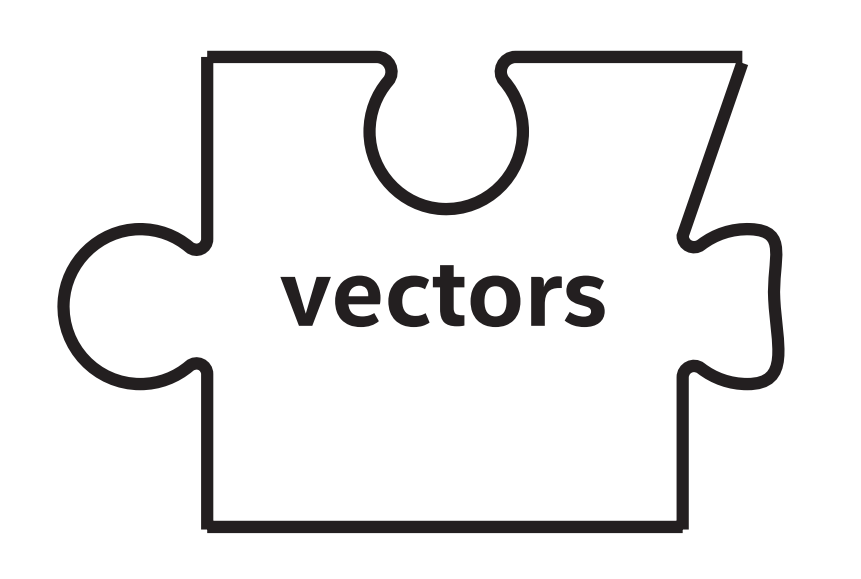
\includegraphics[width=0.3\textwidth]{content/chapter-11/images/1}
\end{center}

向量是数据的集合,计算机中的并行性来自于计算硬件的集合,数据通常以相关的分组进行处理(例如,RGB像素中的颜色通道)。如此重要的特性,值得用一章来讨论向量类型的优点,以及如何使用它们。本章中,不会深入到向量化,因为它会根据设备类型和实现而变化。向量化将在第15和16章中讨论。\par

本章旨在解决以下问题:\par

\begin{itemize}
	\item 什么是向量类型?
	\item 关于向量接口,需要知道多少?
	\item 应该使用向量类型来表示并行性吗?
	\item 什么时候使用向量类型?
\end{itemize}

我们将使用代码示例讨论可用向量类型的优缺点,并重点介绍向量类型的使用。\par




























